%!TEX root = ../prueba.tex

\begin{figure}[hbtp!]
	\begin{center}
		\fbox{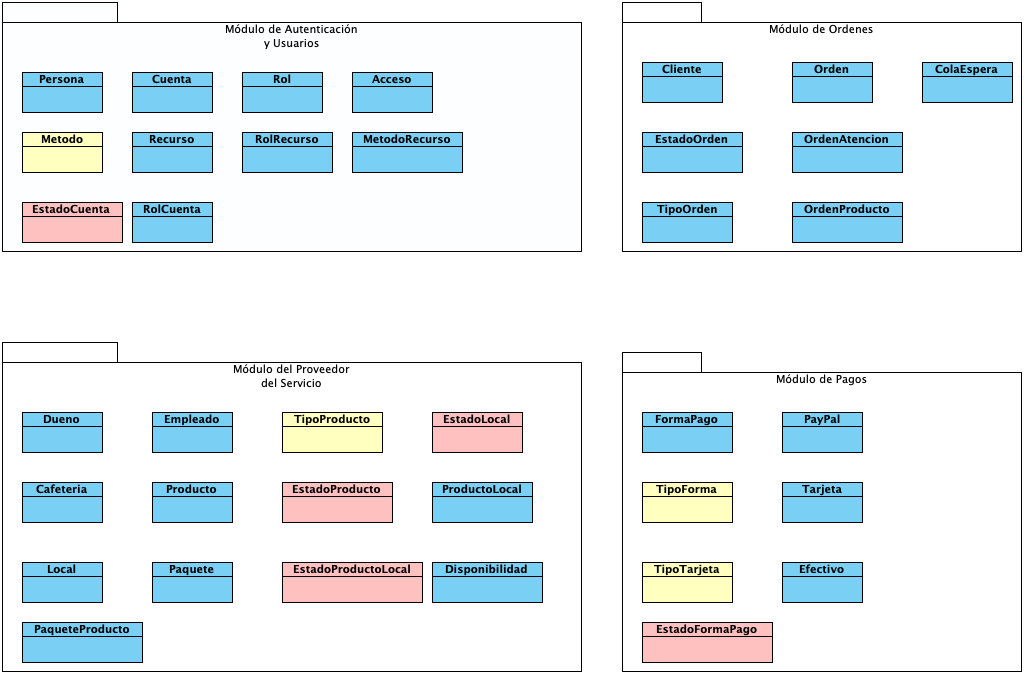
\includegraphics[width=0.5\textwidth]{img/MDI}}
		\caption{Modelo de Información del Sistema}
		\label{fig:mdi}
	\end{center}
\end{figure}
Como se puede observar en la figura \ref{fig:mdi}, el sistema está dividido por módulos, sus entidades serán descritas a continuación por medio de tablas además de que cada módulo se divide por secciones. Los atributos que no están presentes en la figura también son descritos a lo largo de este capítulo.

\section{Módulo de Autenticación y Usuarios}

En el módulo de autenticación y usuarios se encuentran aquellas entidades que permiten el acceso y registro al sistema.

\begin{figure}[hbtp!]
	\begin{center}
		\fbox{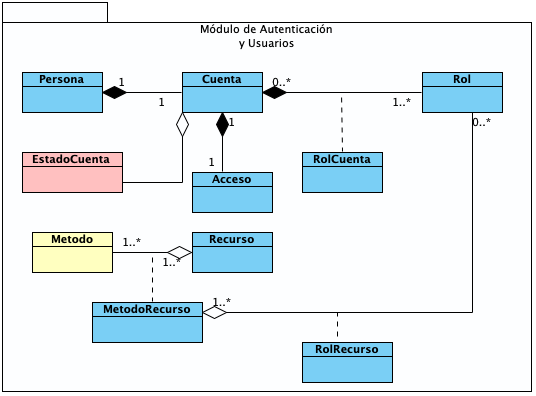
\includegraphics[width=0.7\textwidth]{img/MDI_MAU}}
		\caption{Modelo de Información del Módulo de Autenticación y Usuarios}
		\label{fig:mdimau}
	\end{center}
\end{figure}

\newpage
\begin{Entidad}{Persona}{Persona}
	\attr{nombre}{Nombre}{String}{ Nombre propio con el cual se identificara la persona.}{\datRequerido}
	\attr{primerApellido}{Primer Apellido}{String}{ Palabra que sigue despues del nombre de la persona. }{\datRequerido}
	\attr{segundoApellido}{Segundo Apellido}{String}{ Palabra que sigue despues del primer apellido de la persona. }{\datRequerido}
	\attr{foto}{Foto}{Byte[]}{ Foto del cliente.}{\datOpcional}
	\EntityRelSection
	\brRel{\brRelComposition}{Cuenta}{Una persona tiene una cuenta  con la que el cliente tendra acceso a la aplicación.}
	\brRel{\brRelComposition}{Persona}{Una persona tiene una cuenta para el ingreso al sistema.}
	\brRel{\brRelGeneralization}{Dueño}{El dueño es una persona}
	\brRel{\brRelGeneralization}{Empleado}{Un Empleado es una persona.}
\end{Entidad}
\newpage
\begin{Entidad}{Cuenta}{Cuenta}
	\attr{nombreDeUsuario}{Nombre de Usuario}{String}{ Palabra con la que se identificara el cliente. }{\datRequerido}
	\attr{correoElectronico}{Correo Electrónico}{String}{ Herramienta necesaria para mantener comunicación entre el usuario y la empresa, de modo que esta pueda brindar su mejor servicio. }{\datRequerido}
	\attr{contrasena}{Contraseña}{String}{ Cadena de caracteres elegidos por el usuario para el ingreso único a su cuenta. }{\datRequerido}
	\attr{fechaDeCreacion}{Fecha de Creación}{Timestamp}{Es la fecha en la cual se creo la cuenta de usuario del cliente. }{\datRequerido}
	\EntityRelSection
	\brRel{\brRelComposition}{Persona}{Una persona tiene una cuenta de usuario que le permite acceder a las funcionalidades del sistema con respecto a su rol.}
	\brRel{\brRelComposition}{Rol}{.}
	\brRel{\brRelComposition}{Acceso}{ El cliente accesa al sistema mediante su cuenta. }
	\brRel{\brRelAgregation}{Estado de Cuenta}{.}
\end{Entidad}

\begin{Entidad}{EstadoDeCuenta}{Estado de Cuenta}
	\attr{nombreDeEstado}{Nombre de Estado}{String}{ Estado en el que se encuentra la cuenta del cliente. }{\datRequerido}
	\EntityRelSection
	\brRel{\brRelComposition}{Cuenta}{ Una cuenta solo podra tener una forma de acceso en la aplicaccion.}

\end{Entidad}

\begin{Entidad}{Acceso}{Acceso}
	\attr{fechaDeUltimoAcceso}{fechaDeUltimoAcceso}{Timestamp}{ Fecha en la que se indicara cual fue la ultima vez que el cliente acceso a la aplicación. }{\datRequerido}
	\attr{numeroIntentos}{Número de Intentos}{Integer}{ Cantidad de veces que el usuario intentó ingresar a su cueta sin éxito alguno. }{\datRequerido}
	\EntityRelSection
	\brRel{\brRelComposition}{Cuenta}{El cliente accesa al sistema mediante su cuenta}
\end{Entidad}


%---------------------
\section{Módulo de Órdenes}
En el módulo de órdenes se le permite al \getElementById[Stakeholder]{Cliente} realizar pedidos a los locales que están registrados en el sistema.\\

\begin{figure}[hbtp!]
	\begin{center}
		\fbox{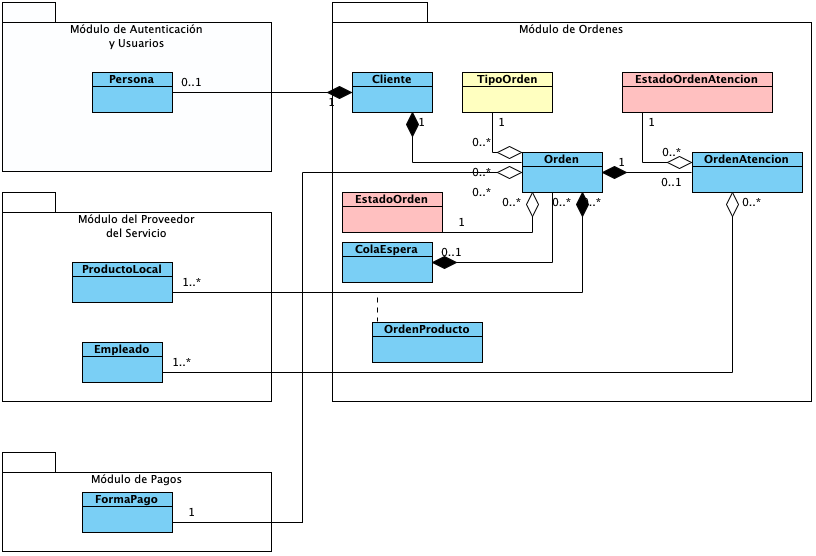
\includegraphics[width=0.5\textwidth]{img/MDI_ORD}}
		\caption{Modelo de Información del Módulo de Órdenes}
		\label{fig:mdiord}
	\end{center}
\end{figure}

\newpage
\begin{Entidad}{cliente}{Cliente}
	\EntityRelSection
	\brRel{\brRelAgregation}{Orden}{ El cliente puede realizar una o varias ordenes a un local.}
	\brRel{\brRelAgregation}{Persona}{Una persona tiene una cuenta para el ingreso al sistema.}
	\brRel{\brRelAgregation}{Forma de Pago}{El cliente podra elegir entre las distintas formas de pago con las que cuenta el sistema.}
\end{Entidad}

\begin{Entidad}{Orden}{Orden}
	\attr{fechaOrden}{Fecha de la Orden}{Date}{ Fecha en la que se realizó la orden. }{\datRequerido}
	\attr{fechaUltimaActualizacion}{Fecha Ultima Actualizacion}{Date}{ Fecha en la que se realizó la ultima modificacion a la Orden. }{\datRequerido}
	\attr{stConfirmacion}{Estado de Confirmación}{Boolean}{ Estado en donde se podra ver si la orden fue confirmada o rechazada. }{\datRequerido}
	\attr{stPrioridad}{Estado de Prioridad}{Integer}{ Estado en donde se vera la priodirad de la orden. }{\datRequerido}
	\EntityRelSection
	\brRel{\brRelComposition}{Cliente}{ El cliente puede realizar una o varias ordenes a un local.}
	\brRel{\brRelComposition}{Cola de Espera}{Una orden sera asignada a una cola de espera.}
	\brRel{\brRelComposition}{Estado de Orden}{ Una o muchas ordenes pueden tener el mismo estado.}
	\brRel{\brRelComposition}{Tipo de Orden}{ Una o muchas ordenes pueden pertenecer al mismo tipo de orden.}
	\brRel{\brRelComposition}{Orden en Atencion}{Una orden puede ser atendiada por un cocinero.}
	\brRel{\brRelComposition}{Producto en orden}{Producto que se encuentra dentro de una orden.}
	\brRel{\brRelComposition}{Produnto}{Un producto puede pertenecer a varias ordenes.}
	\brRel{\brRelAgregation}{Local}{Muchas ordenes pueden ser dirijidas a un local.}
\end{Entidad}

\begin{Entidad}{colaEspera}{Cola de Espera}
	\attr{fechaCola}{Fecha de Cola}{Date}{ Fecha en la que se inicio la cola de espera. }{\datRequerido}
	\attr{ultimaActualizacion}{Fecha Ultima Actualizacion}{Timestamp}{ Fecha de la actualizacion del estado de la cola de espera.}{\datRequerido}
	\EntityRelSection
	\brRel{\brRelComposition}{Orden}{Una orde sera asignada a una cola de espera.}
\end{Entidad}

\begin{Entidad}{estadoOrden}{Estado de Orden}
	\attr{nombreEstado}{Nombre del Estado}{String}{Estado en que se encuentra a Orden. }{\datRequerido}
	\EntityRelSection
	\brRel{\brRelAgregation}{Orden}{ Una o muchas ordenes pueden tener el mismo estado.}
\end{Entidad}

\begin{Entidad}{tipoOrden}{Tipo de Orden}
	\attr{nombreTipo}{Nombre del Tipo}{String}{ Tipo de Orden que se realizó. }{\datRequerido}
	\EntityRelSection
	\brRel{\brRelAgregation}{Orden}{Una o muchas ordenes pueden ppertenecer al mismo tipo de orden}
\end{Entidad}

\begin{Entidad}{ordenAtencion}{Orden en Atención}
	\EntityRelSection
	\brRel{\brRelComposition}{Orden}{Una orden debe ser atendida por un cocinero.}
	\brRel{\brRelAgregation}{Estado de Orden en Atención}{}
\end{Entidad}

\begin{Entidad}{estadoOrdenAtencion}{Estado de Orden en Atención}
	\attr{nombreEstado}{Nombre del Estado}{String}{ }{\datRequerido}
	\EntityRelSection
	\brRel{\brRelAgregation}{Orden en Atención}{}
\end{Entidad}

\begin{Entidad}{productoOrden}{Producto en Orden}
	\attr{comentario}{Comentario}{String}{ Comentario acerca del producto  }{\datRequerido}
	\attr{comentarioCalificacion}{Comentario de Calificación}{String}{ Calificacion con un intervalo de 0 a 5 acerca del producto  }{\datRequerido}
	\attr{nuRating}{Numero Rating}{Double}{ Numero en el que estara posicionado el producto, esto depende de la calificacion dada por los clientes. }{\datRequerido}
	\EntityRelSection
	\brRel{\brRelComposition}{Orden}{Producto que se encuentra dentro de una orden}
	\brRel{\brRelComposition}{Producto}{Producto al cual se le dara una calificación y un rating}
\end{Entidad}

%------------------------
\section{Modelo de Información del Módulo del Proveedor del Servicio}

En el módulo del proveedor del servicio se le permitee al \getElementById[Stakeholder]{Jefe} registrar en el sistema la información de cafeterías, de sus locales y de los productos que se ofertan en esos locales. Así mismo el \getElementById[Stakeholder]{ResponsableDeLocal} puede registrar la información de productos que se oferten únicamente en un local.

\begin{figure}[hbtp!]
	\begin{center}
		\fbox{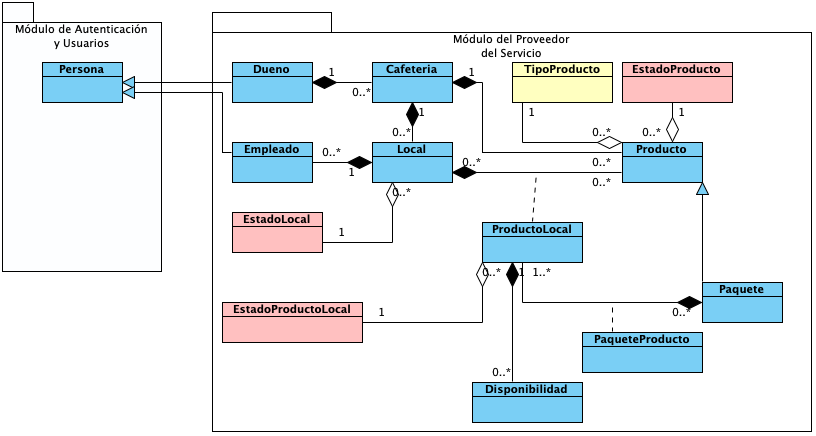
\includegraphics[width=0.5\textwidth]{img/MDI_MPS}}
		\caption{Modelo de Información del Módulo del Proveedor del Servicio}
		\label{fig:mdimps}
	\end{center}
\end{figure}

\newpage
\begin{Entidad}{dueño}{Dueño}
	\EntityRelSection
	\brRel{\brRelComposition}{Cafetería}{El dueño puede agregar una o muchas cafeterías al sistema}
	\brRel{\brRelGeneralization}{Persona}{El dueño es una persona}
\end{Entidad}

\begin{Entidad}{estadoProducto}{Estado de Producto}
	\attr{nombreEstado}{Nombre de Estado}{String}{ Estado en que se encuentra el producto. }{\datRequerido}
	\EntityRelSection
	\brRel{\brRelAgregation}{Producto}{Un estado de producto puede ser asignado a uno o muchos productos.}
\end{Entidad}
\newpage
\begin{Entidad}{cafeteria}{Cafetería}
	\attr{nombreCafeteria}{Nombre de Cafeteria}{String}{ Nombre con el cual se identificara la cafetería }{\datRequerido}
	\EntityRelSection
	\brRel{\brRelAgregation}{Producto}{ Una cafeteria puede tener uno o mas Productos a la venta para los clientes.}
	\brRel{\brRelComposition}{Dueño}{El dueño puede agregar una o muchas cafeterías al sistema}
	\brRel{\brRelComposition}{Local}{Una cafetería puede tener muchos locales.}
\end{Entidad}

\begin{Entidad}{tipoProducto}{Tipo Producto}
	\attr{tipo}{Tipo}{String}{ El el tipo al que pertenece el producto. }{\datRequerido}
	\EntityRelSection
	\brRel{\brRelAgregation}{Producto}{Muchos productos pueden pertenecer al mismo tipo.}
\end{Entidad}

\begin{Entidad}{producto}{Producto}
	\attr{nombreProducto}{Nombre del Producto}{String}{ Nombre con el cual se identificara el producto. }{\datRequerido}
	\attr{nuPrecioVenta}{Precio de Venta}{Double}{ Precio de venta que se le asignara al producto.}{\datRequerido}
	\attr{nuPrecioCompra}{Precio de Compra}{Double}{ Precio de compra que se le asignara al producto.}{\datRequerido}
	\EntityRelSection
	\brRel{\brRelComposition}{Cafetería}{ Un producto solo puede tener una cafetería.}
	\brRel{\brRelAgregation}{Estado de producto}{Un estado de produnto puede ser asignado a uno o muchos productos}
	\brRel{\brRelAgregation}{Tipo de Producto}{Muchos productos pueden pertenecer al mismo tipo.}
	\brRel{\brRelComposition}{Producto en Orden}{Producto al cual se le dara una calificacon y un rating.}
	\brRel{\brRelComposition}{Orden}{Un producto puede pertenecer a varias ordenes.}
	\brRel{\brRelGeneralization}{Producto de Local}{Un producto es aquel que se encuentra dentro de un local}
\end{Entidad}

\begin{Entidad}{estadoLocal}{Estado del Local}
	\attr{nombreEstado}{Nombre del Estado}{String}{ Estado en el que se encuetra el local. }{\datRequerido}
	\EntityRelSection
	\brRel{\brRelAgregation}{Local}{ Varios locales pueden pertenecer al mismo estado.}
\end{Entidad}

\begin{Entidad}{local}{Local}
	\attr{nombreLocal}{Nombre del Local}{String}{ Nombre con el que se identificara el Local }{\datRequerido}
	\attr{nuRating}{Rating}{Integer}{ Rating que tiene el local, esto depende de la calificacion que le den los clientes. }{\datRequerido}
	\attr{nuLongitud}{Longitud}{Double}{ Cordenadas geograficas del local. }{\datRequerido}
	\attr{nuLatitud}{Latitud}{Double}{ Cordenadas geograficas del local. }{\datRequerido}
	\attr{foto}{Foto}{Byte[]}{ Foto del Local para que el cliente pueda identificarlo.}{\datRequerido}
	\attr{horaInicio}{Hora de Inicio}{Time}{ Hora en la que el Local comienza a dar servicio.}{\datRequerido}
	\attr{horaFin}{Hora de Fin}{Time}{ Hora en la que el Local termina de dar servicio.}{\datRequerido}
	\EntityRelSection
	\brRel{\brRelComposition}{Cafetería}{Una cafetería puede tener muchos locales.}
	\brRel{\brRelAgregation}{Producto de Local}{Un local puede contar con ningun o productos.}
	\brRel{\brRelAgregation}{Orden}{Muchas ordenes pueden ser dirijidas a un local.}
	\brRel{\brRelComposition}{Responsable}{Solo habra un responsable en el local.}
	\brRel{\brRelComposition}{Empleado}{Varios empreados pueden estar asignados a un local.}
\end{Entidad}

\begin{Entidad}{productoLocal}{Producto del Local}
	\EntityRelSection
	\brRel{\brRelComposition}{Paquete}{Un paquete puede estar compuesto por varios productos.}
	\brRel{\brRelComposition}{Producto en paquete}{Producto que esta dentro de un paquete.}
	\brRel{\brRelGeneralization}{Producto}{Un producto es aquel que se encuentra dentro de un local.}
	\brRel{\brRelGeneralization}{Paquete}{Un paquete es un producto que esta dentro de un local.}
	\brRel{\brRelAgregation}{Estado Producto de Local}{Muchos productos del local pueden ser aasignados al mismo estado}
	
\end{Entidad}

\begin{Entidad}{empleado}{Empleado}
	\EntityRelSection
	\brRel{\brRelComposition}{Local}{Varios empleados pueden estar asignados a un local.}
	\brRel{\brRelGeneralization}{Persona}{Un espleado es una persona.}
	\brRel{\brRelGeneralization}{Orden de Atención}{Un empleado puede atender una orden.}
\end{Entidad}

\begin{Entidad}{responsable}{Responsable}
	\EntityRelSection
	\brRel{\brRelComposition}{Local}{Solo habra un responsable en el local.}
	\brRel{\brRelGeneralization}{Empleado}{El responsable es un empleado}
\end{Entidad}

\begin{Entidad}{estadoProductoLocal}{Estado Producto de Local}
	\attr{nombreEstado}{Nombre del Estado}{String}{ Estado en que se encuentra el producto. }{\datRequerido}
	\EntityRelSection
	\brRel{\brRelAgregation}{Producto de Local}{Muchos productos del local pueden ser aasignados al mismo estado}
\end{Entidad}

\begin{Entidad}{productoPaquete}{Producto en Paquete}
	\EntityRelSection
	\brRel{\brRelComposition}{Paquete}{Producto que esta dentro de un paquete}
	\brRel{\brRelComposition}{Producto de Local}{}
\end{Entidad}

\begin{Entidad}{paquete}{Paquete}
	\EntityRelSection
	\brRel{\brRelComposition}{Producto local}{Un paquete puede estar compuesto por varios productos}
	\brRel{\brRelGeneralization}{Producto de Local}{El paquete es un producto que esta en el local.}
\end{Entidad}

%--------------
\section{Modelo de Información del Módulo de Pagos}

En el módulo de pagos se le permite al \getElementById[Sstakeholder]{Cliente} agregar, editar o eliminar los métodos con los que puede realizar el pago de sus ordenes.

\begin{figure}[hbtp!]
	\begin{center}
		\fbox{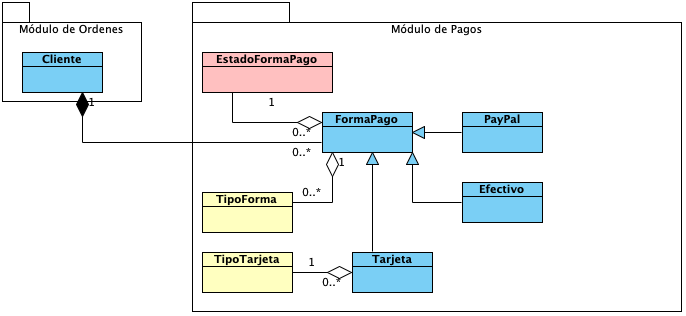
\includegraphics[width=0.5\textwidth]{img/MDI_PGS}}
		\caption{Modelo de Información del Módulo de Pagos}
		\label{fig:mdimpg}
	\end{center}
\end{figure}

\newpage
\begin{Entidad}{tipoForma}{Tipo de Forma de Pago}
	\attr{nombreTipo}{Nombre del Tipo}{String}{ Nombre con el que se identificara el tipo de pago. }{\datRequerido}
	\EntityRelSection
	\brRel{\brRelAgregation}{Forma de Pago}{Varias formas de pago pueden ser del mismo tipo.}
\end{Entidad}

\begin{Entidad}{paypal}{Paypal}
	\attr{correoElectronico}{Correo Electronico}{String}{ Correo electronico con el cual se registro en el sistema.}{\datRequerido}
	\attr{contraseña}{Contraseña}{String}{ Contraseña del usuario que utilza para acceder al sistema.}{\datRequerido}
	\EntityRelSection
	\brRel{\brRelGeneralization}{Forma de Pago}{Paypal es una forma de pago con la que se puedo realizar la compra de un producto.}
\end{Entidad}

\begin{Entidad}{formaPago}{Forma de Pago}

	\EntityRelSection
	\brRel{\brRelComposition}{Cliente}{Un cliente tiene una o varias formas de pago.}
	\brRel{\brRelAgregation}{Orden}{Una orden puede se puede pagar por varias formas de pago.}
	\brRel{\brRelAgregation}{Tipo de Forma de Pago}{Varias formas de pago pueden ser del mismo tipo.}
	\brRel{\brRelGeneralization}{Efectivo}{El efectivo es una forma de pago con la que se puede realizar la compra de un producto}
	\brRel{\brRelGeneralization}{Paypal}{Payoal es una forma de pago con la que se puede realizar la compra de un producto}
	\brRel{\brRelGeneralization}{Tarjeta}{El uso de la tarjeta de credito es una forma de pago con la que se puede realizar la compra de un producto}
\end{Entidad}

\begin{Entidad}{efectivo}{Efectivo}
	\EntityRelSection
	\brRel{\brRelGeneralization}{Forma de Pago}{El efectivo es una forma de pago con la que se puede realizar la compra de un producto}
\end{Entidad}

\begin{Entidad}{tarjeta}{Tarjeta}
	\attr{numeroTarjeta}{Numero de Tarjeta}{String}{ 16 digitos para la identificacion de la tarjeta. }{\datRequerido}
	\attr{fechaVencimiento}{Fecha de Vencimiento}{Date}{ Fecha en la que la tarjeta expira}{\datRequerido}
	\attr{claveSeguridad}{Clave de Seguridad}{String}{ Calve unica para la verificacion de los datos de la tarjeta.}{\datRequerido}
	\EntityRelSection
	\brRel{\brRelGeneralization}{Forma de pago}{El uso de la tarjeta de credito es una forma de pago con la que se puedo realizar la compra de un producto.}
	\brRel{\brRelAgregation}{Tarjeta}{Una Tarjeta tiene solo un tipo de tajeta.}
\end{Entidad}

\begin{Entidad}{tipoTarjeta}{Tipo de Tarjeta}
	\attr{nombreTipo}{Nombre del Tipo}{String}{ Nombre del tipo de tarjeta que se esta utilizando }{\datRequerido}
	\EntityRelSection
	\brRel{\brRelAgregation}{Tarjeta}{Una Tarjeta tiene solo un tipo de tajeta.}
\end{Entidad}


